\documentclass{article}
\textheight 23.5cm \textwidth 15.8cm
%\leftskip -1cm
\topmargin -1.5cm \oddsidemargin 0.3cm \evensidemargin -0.3cm
%\documentclass[final]{siamltex}

\usepackage{verbatim}
\usepackage{fancyhdr}
\usepackage{graphicx}

%\pagestyle{fancy} \lhead{FDM Homework Template} \chead{}
%\rhead{\bfseries Yan XU}
%
%\lfoot{} \cfoot{} \rfoot{\thepage}
%\renewcommand{\headrulewidth}{0.4pt}
%\renewcommand{\footrulewidth}{0.4pt}
%

%利用TEX排版系统的CTEX中文套装
\usepackage[UTF8,noindent]{ctex}
%等式对齐
\usepackage{amsmath}
\usepackage{amssymb}

\title{MiniDraw}
\author{陈柯}

\begin{document}
	\maketitle
	
	\section{目的}
	
	制作画图小工具 MiniDraw。
	\section{类图展示}
	\begin{figure}[htb]
		\begin{center}
		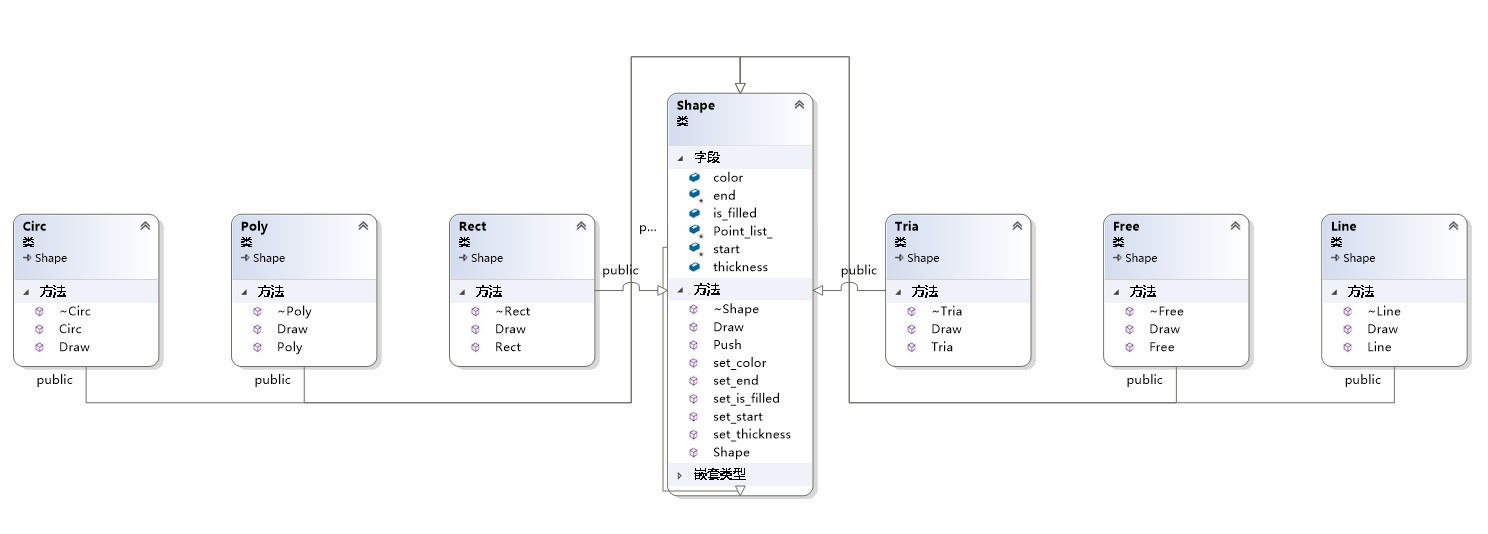
\includegraphics[width=7in]{class1.jpg}
		\end{center}
	\end{figure}
	\clearpage
	\begin{figure}[htb]
		\begin{center}
			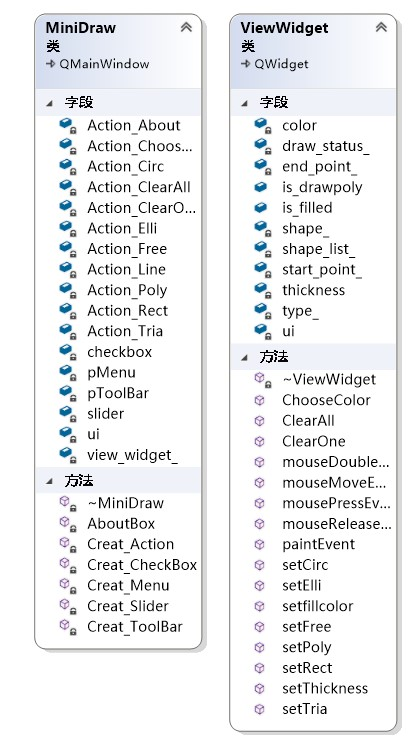
\includegraphics[width=3.5in]{class2.jpg}
		\end{center}
	\end{figure}

	\section{实现功能介绍}
	\subsection{按键功能介绍}
	\begin{table}[h]
		\centering
		\caption{各按键的功能}
		\begin{tabular}{ | c | l | }
			\hline
			按键 & 功能 \\ \hline
			\begin{minipage}[b]{0.1\columnwidth}
				\centering
				\raisebox{-.5\height}{
\includegraphics[width=\linewidth]{Line.png}}
			\end{minipage}
			& 画直线\\\hline
			
			\begin{minipage}[b]{0.1\columnwidth}
				\centering
				\raisebox{-.5\height}{
\includegraphics[width=\linewidth]{Tria.png}}
			\end{minipage}
			& 画一条边水平的三角形\\\hline
			
			\begin{minipage}[b]{0.1\columnwidth}
				\centering
				\raisebox{-.5\height}{
\includegraphics[width=\linewidth]{Rect.png}}
			\end{minipage}
			& 画矩形\\\hline
			
			\begin{minipage}[b]{0.1\columnwidth}
				\centering
				\raisebox{-.5\height}{
\includegraphics[width=\linewidth]{Circ.png}}
			\end{minipage}
			& 画圆形\\\hline
			
			\begin{minipage}[b]{0.1\columnwidth}
				\centering
				\raisebox{-.5\height}{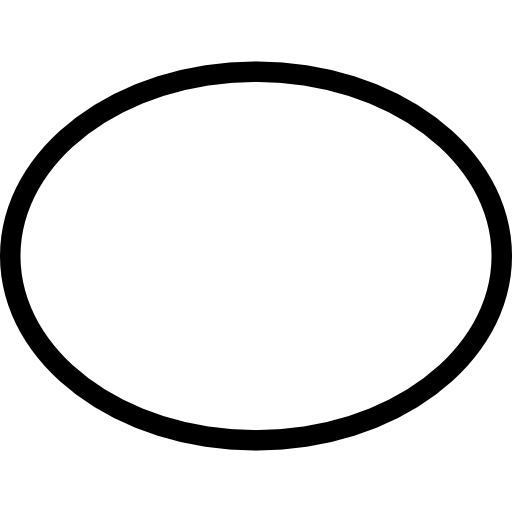
\includegraphics[width=\linewidth]{Elli.png}}
			\end{minipage}
			& 画椭圆\\\hline
			
			\begin{minipage}[b]{0.1\columnwidth}
				\centering
				\raisebox{-.5\height}{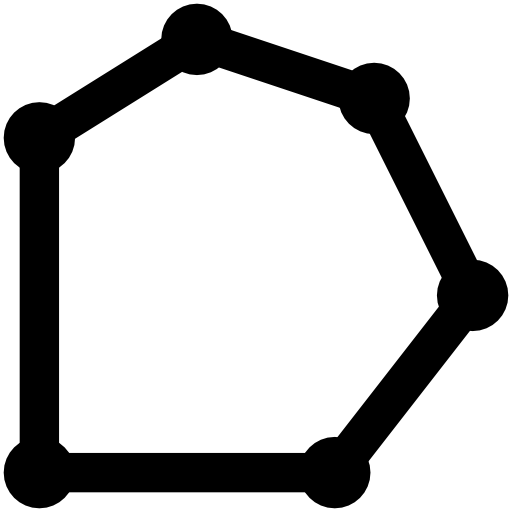
\includegraphics[width=\linewidth]{Poly.png}}
			\end{minipage}
			& 画多边形,双击自动封闭\\\hline
			
			\begin{minipage}[b]{0.1\columnwidth}
				\centering
				\raisebox{-.5\height}{
\includegraphics[width=\linewidth]{Free.png}}
			\end{minipage}
			& 自由画笔\\\hline
			
			\begin{minipage}[b]{0.1\columnwidth}
				\centering
				\raisebox{-.5\height}{
\includegraphics[width=\linewidth]{ChooseColor.png}}
			\end{minipage}
			& 挑选需要绘制的颜色\\\hline
			
			\begin{minipage}[b]{0.1\columnwidth}
				\centering
				\raisebox{-.5\height}{
\includegraphics[width=\linewidth]{SmallEraser.png}}
			\end{minipage}
			& 擦除最后一个绘制的图形\\\hline
			
			\begin{minipage}[b]{0.1\columnwidth}
				\centering
				\raisebox{-.5\height}{\includegraphics[width=\linewidth]{bigEraser.png}}
			\end{minipage}
			& 擦除所有图形\\\hline
			
			\begin{minipage}[b]{0.08\columnwidth}
				\centering
				\raisebox{-.5\height}{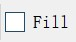
\includegraphics[width=\linewidth]{checkbox.jpg}}
			\end{minipage}
			& 通过勾选确定是否图形需要填充颜色\\\hline
			
			\begin{minipage}[b]{0.08\columnwidth}
				\centering
				\raisebox{-.5\height}{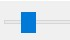
\includegraphics[width=\linewidth]{slider.jpg}}
			\end{minipage}
			& 通过滑条挑选笔的粗细\\\hline
		\end{tabular}
	\end{table}
	
	
	\clearpage
	\subsection{界面设计}
	\begin{figure}[htb]
		\begin{center}
		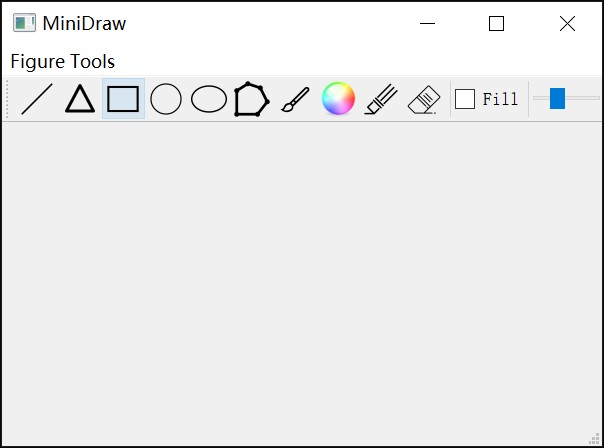
\includegraphics[width=4in]{UI.jpg}
		\end{center}
	\end{figure}
	\subsection{几何形状绘制}
	可以绘制直线,三角形,圆形,矩形,椭圆,多边形。
	\begin{figure}[htb]
		\begin{center}
			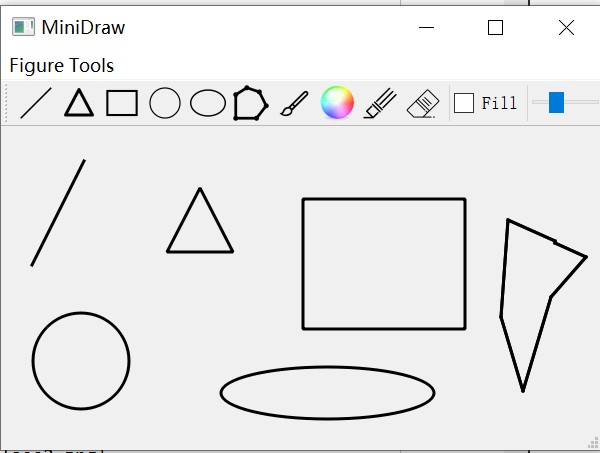
\includegraphics[width=4in]{geo.jpg}
		\end{center}
	\end{figure}
	\clearpage
	也可以使用画笔自由绘制。
	\begin{figure}[htb]
		\begin{center}
			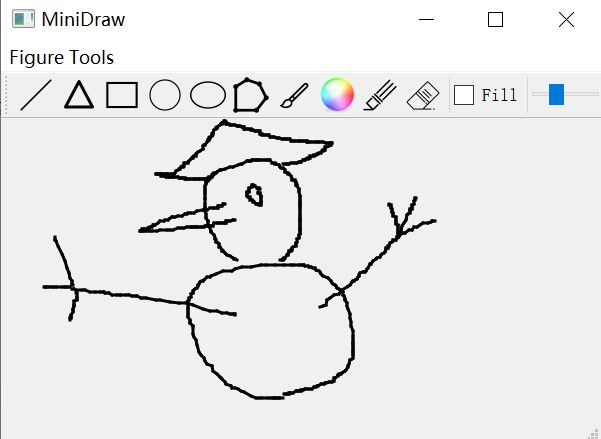
\includegraphics[width=4in]{draw.jpg}
		\end{center}
	\end{figure}
	
	可以挑选颜色和填充颜色。
	\begin{figure}[htb]
		\begin{center}
			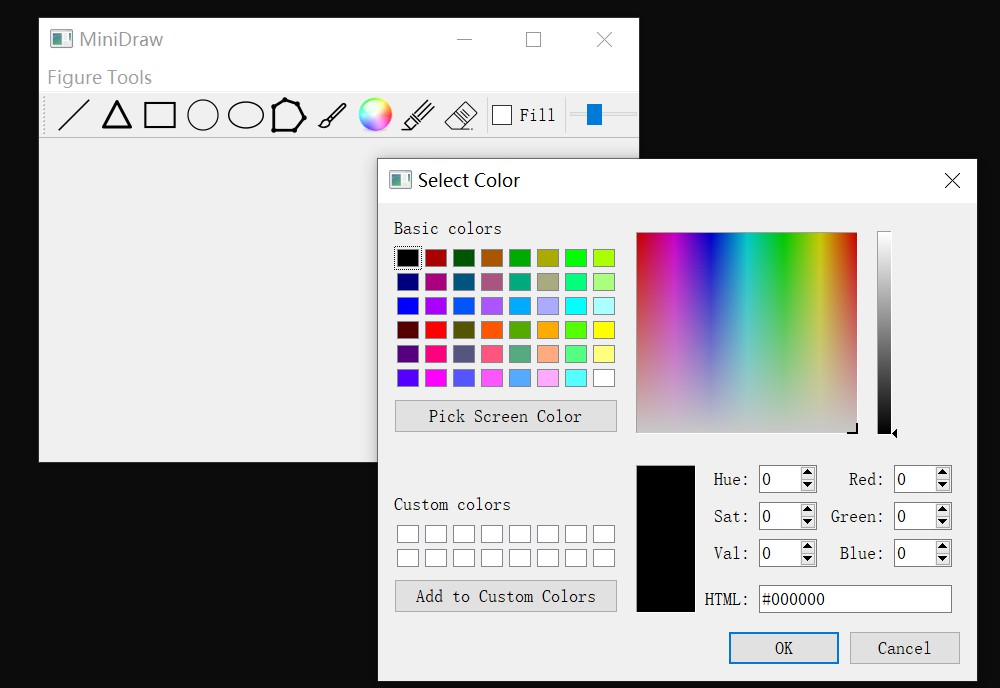
\includegraphics[width=4in]{colorui.jpg}
		\end{center}
	\end{figure}\clearpage
	\begin{figure}[htb]
		\begin{center}
			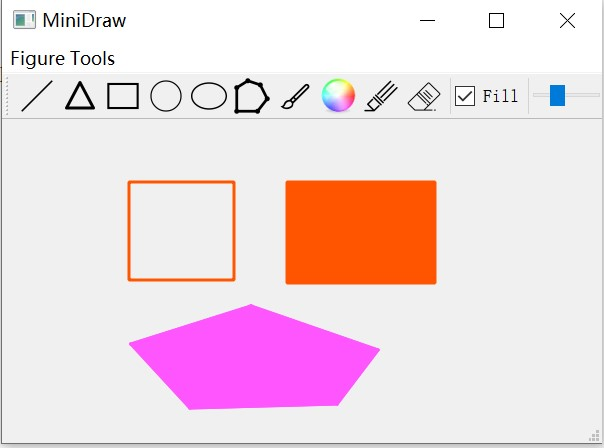
\includegraphics[width=4in]{color.jpg}
		\end{center}
	\end{figure}

	可以挑选笔的粗细。
	\begin{figure}[htb]
		\begin{center}
			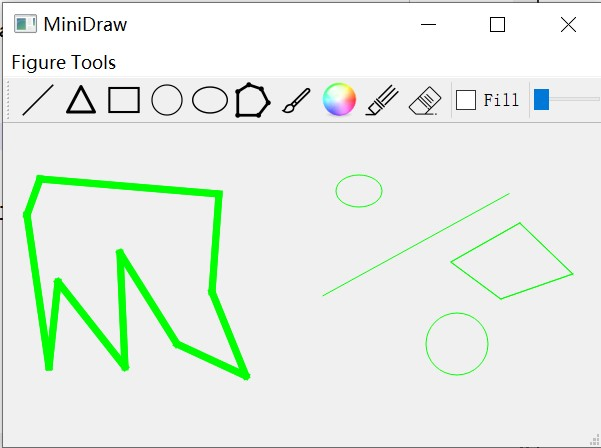
\includegraphics[width=4in]{thick.jpg}
		\end{center}
	\end{figure}
	

\end{document}
